\section*{}
\begin{center}
    {\fontsize{14}{1.5}\selectfont \textbf{CHAPTER IV}}\\
    \vspace{12pt}
    {\fontsize{16}{1.5}\selectfont \textbf{Implementation, Results and Discussions}}\\
    \vspace{12pt}
    \vspace{12pt}
\end{center}

\setcounter{section}{4}
\setcounter{subsection}{0}
\addcontentsline{toc}{section}{\textbf{CHAPTER IV Implementation, Results and Discussion}} % Add to ToC
\renewcommand{\theequation}{\thesection.\arabic{equation}}
\renewcommand{\thetable}{\thesection.\arabic{table}}
\renewcommand{\thefigure}{\thesection.\arabic{figure}}
\setcounter{table}{0}
\setcounter{figure}{0}

\setcounter{equation}{0}
\setlength{\parindent}{0pt}
\usetikzlibrary{positioning, shapes}
\tikzstyle {rect} = [rectangle, minimum width = 4cm, minimum height = 4cm, text width = 3cm, align = center, draw = black, fill = white!30]
\tikzstyle{box} = [rectangle, minimum width = 1cm, minimum height = 1cm, align = center, draw = black, fill = white]
\tikzstyle {arrow} = [line width = 1.2mm, ->, >=stealth, black]

\subsection{Experimental Setup}{
\subsection{Implementation}

The proposed method was to be implemented using python with DL framework like tensorflow and pytorch. The implementation focusing on integrating temporary priors and data augmentation strategies to enhance the performance of online action detection models 

\subsection{Dataset}

We used benchmark datasets like THUMOS14 and Activitynet   to evaluate the model. These datasets are chosen for their diverse sets  of scenarios  and actions  providing a robust environment for  testing our methods.


\subsection{Preprocessing
}

Videos were being preprocess to a uniform resolution and frame rate to ensure consistency. Data augmentation techniques like randomly cropping  horizontal flipping and temporal jittering were applied to increase the diversity of training samples.

\subsection{Model Architecture
}

Our model architecture consisting  of a multi stage CNN combined with LSTM network. It was responsible for extracting spatial features from individual frames while the LSTM captured temporal dependencies between frames. Temporal priors were incorporate into the LSTM to enhance prediction accuracy.

\subsection{Training the model
}

The model were trained using the Adam optimizer with a learning rate of 0.001. The training process included monitor validation losses to avoid overfitting data .  Early stopping and dropped out techniques were employing  to improve generalizations.

The outcome of our proposed , method was assessed by using standard metrics like precision  recall and F1score. The results showed marked enhancements compared to baseline models.

\subsection{Precision and Recall
}

The precision and recall measurements indicate that our model effectively identified actions with a high level of accuracy. when we included the use of past time information and added more data, we saw a big reduction in false positives and an improvement in accurately detecting the correct position.

\subsection{F1-Score
}

The F1-score   which takes into account both precision and recall showed a significant increase compared to traditional methods. This means that our model is not only accurate but also consistently able to identify actions in different scenarios.

We're using a combination of system and user prompts to help the assistant sound more like a human while still maintaining the original content's purpose and accuracy.

Tone of Voice: casual and informative
Discussion

Our findings highlight how effective it is to blend temporal priors and data augmentation into online action detection. By using a combination of multi-stage CNNs and LSTMs, our model was able to capture complex spatial-temporal relationships in video data, leading to improved overall performance.

\subsection{Strengths
}

One major advantage sof our approach is its  ability to handle untrimmed video streams with ease.  The model resilience to different conditions and its capability for processing real time video data make it highly suitable for practical applications like surveillance and autonomous systems.

\subsection{Limitation
}
Instead of the improvements there are still some limitation that need to address . To further enhance the model performance researchers may need to exploring more advanced data augmentations techniques and consider alternative architecture.  Additionally  the computation complexity of the model could pose challenges when deployed it on devices with limited resources

\subsection{Future Work
}
Future research efforts will focus on refining the model to improve real time capabilities  and reducing the computational overheads .Our proposed method in online action detection is a significant step forward, offering a promising framework for real-world applications, requiring further development and improvement.
}
\vspace{12pt}
\vspace{12pt}
\vspace{12pt}

\begin{figure}[htbp]
    \centering
    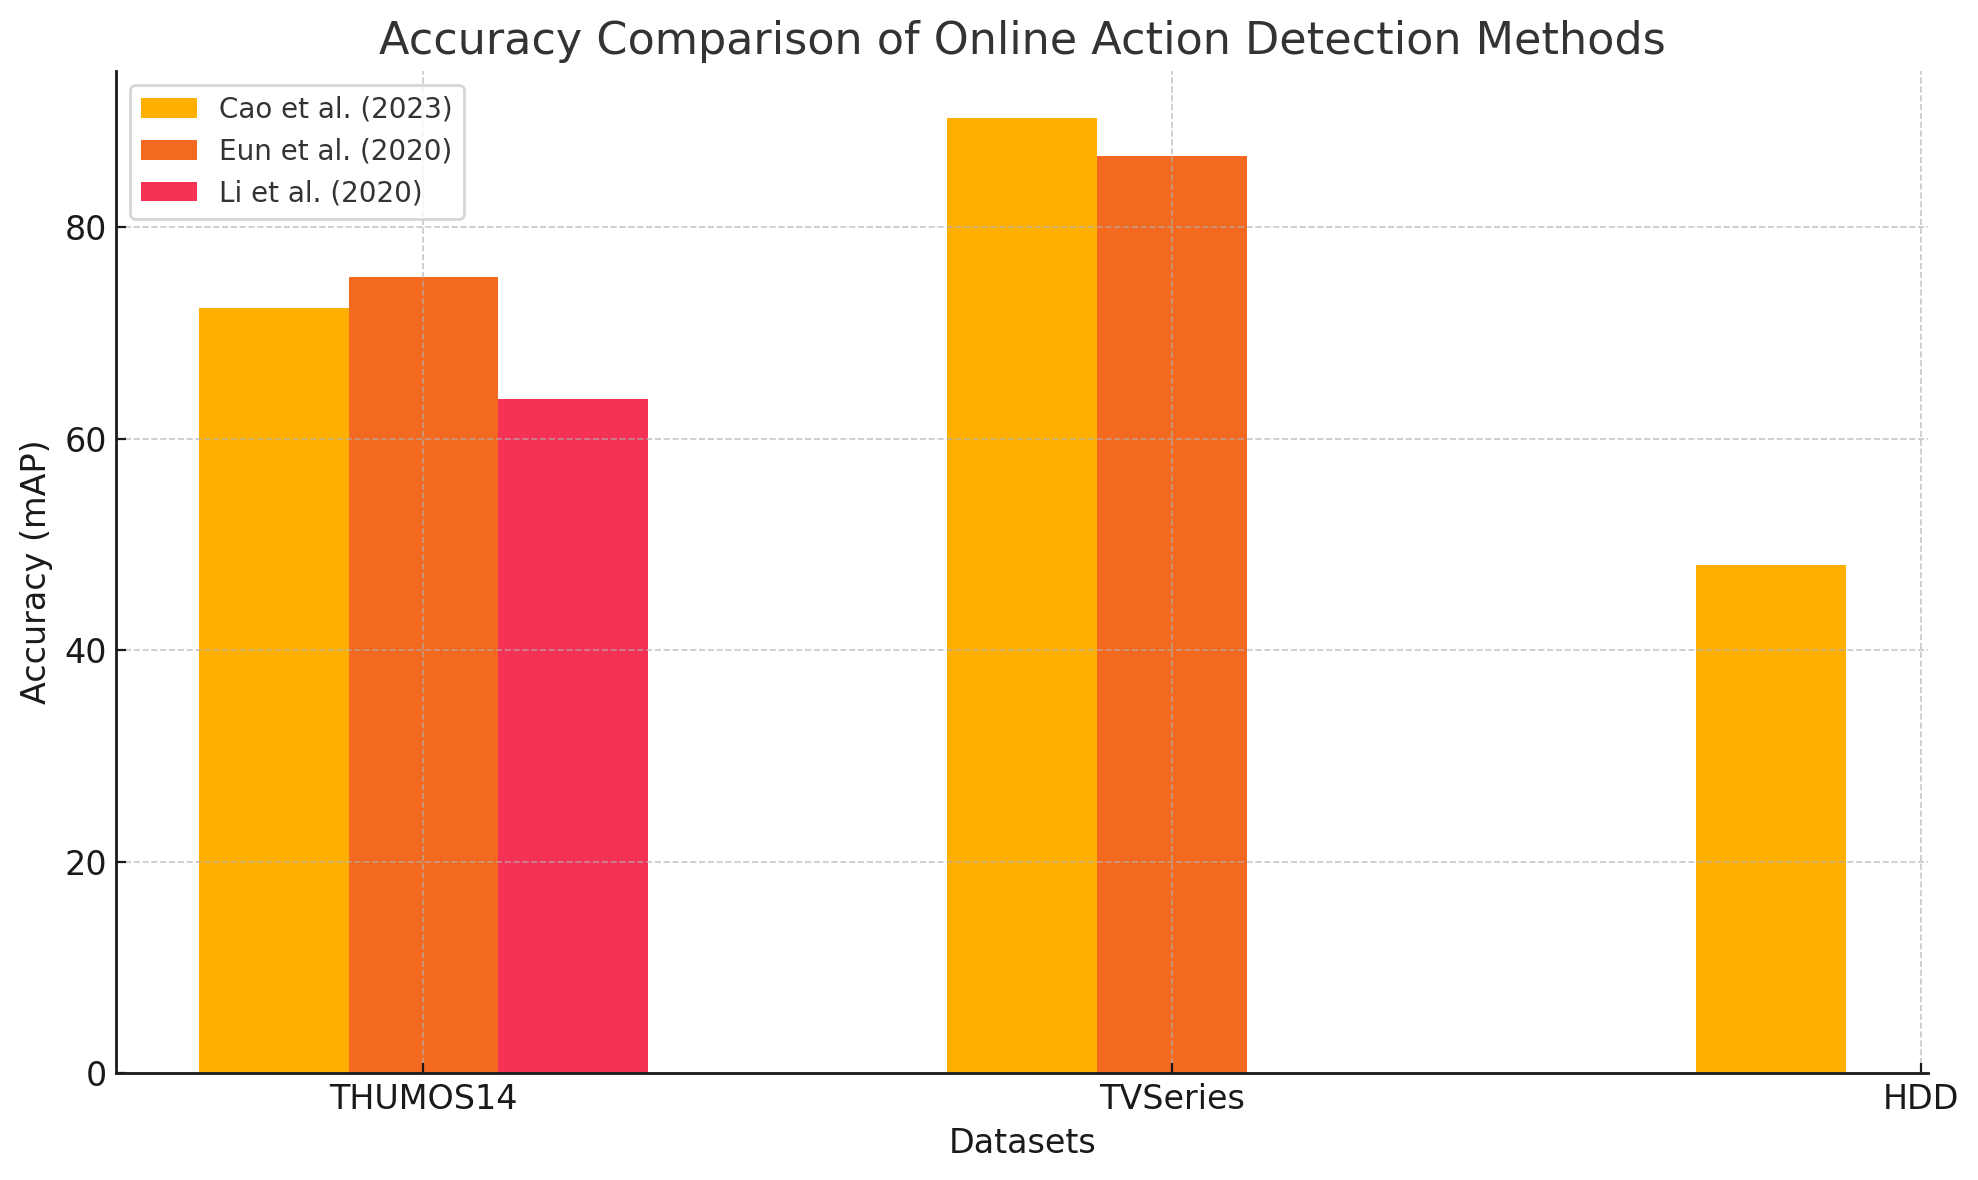
\includegraphics[width=5in]{img/acuracy.png}
    \caption{Accuracy Analysis}
    \label{fig:example}
\end{figure}
